\section{Sea-Level Fingerprints (GRACE)}
\subsection{Goals} %{{{
\begin{itemize}
	\item Setup a ISSM-SESAW model with GRACE-based forcing
	\item Run the model to compute sea-level fingerprints
\end{itemize}

Go to \verb@trunk/examples/SlrGRACE/@ to do this tutorial.

%}}}
\subsection{Mesh} %{{{
Set \verb@steps=1@ to create an unstructured global mesh. Choose \verb@mindistance_coast@,
\verb@mindistance_lan@, and \verb@maxdistance@ as you wish for generating a mesh. The nominal
parameters should generate the following mesh:
\begin{figure}[H]
	\begin{center}
		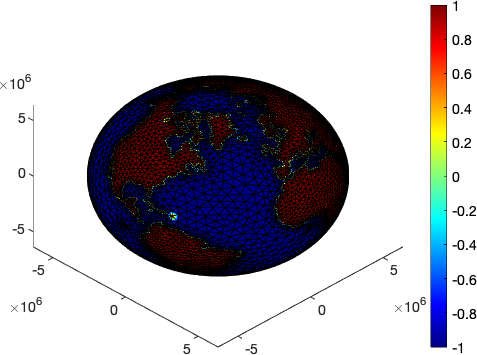
\includegraphics[scale=2.8]{/assets/img/tutorials/sealevelfingerprints/Mesh.png}
	\end{center}
\end{figure}
%}}}
\subsection{GRACE loads} %{{{
Set \verb@steps=2@ to load GRACE-based estimate of water equivalent height (WEH) change for a chosen
month. Choose \verb@year_month@ as you wish. The nominal month is January 2007 and here is the load
model (cf. \verb@steps=5@ for plotting):
\begin{figure}[H]
	\begin{center}
		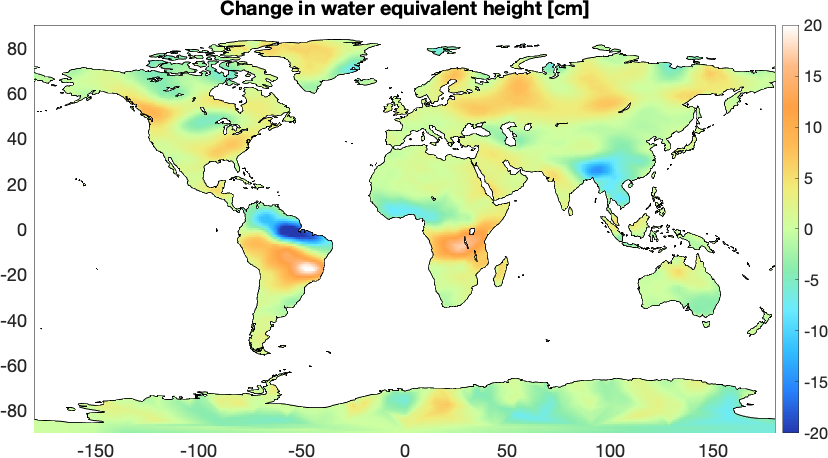
\includegraphics[scale=2]{/assets/img/tutorials/sealevelfingerprints/Weh.png}
	\end{center}
\end{figure}
%}}}
\subsection{Parameterization} %{{{
In the next step, you will load the Earth model. The nominal model is PREM; \verb@lovenumbers@ reads
the associated Love numbers. You will also have to set up some standard parameters regarding ice
sheets for passing the consistency.
%}}}
\subsection{Solve Model} %{{{
In \verb@steps=4@, you will choose the solid-Earth physics (e.g., gravitation, viscoelasticity, and
rotation) that you wish to consider. You may also request model outputs (e.g., sea level and bedrock
motion). You must set \verb@masstransport@ and \verb@slc@ flags on before solving the \verb@transient@
model. See \verb@steps=6@ for running a model with multiple (transient) loads.
%}}}
\subsection{Some Results} %{{{
Once the model run is completed, you may plot results. Some useful plotting scripts are located in
\verb@steps=5@ and \verb@steps=7@. In the latter, you can also find a script to make an animation.
Here is an example result for January 2007:
\begin{figure}[H]
	\begin{center}
		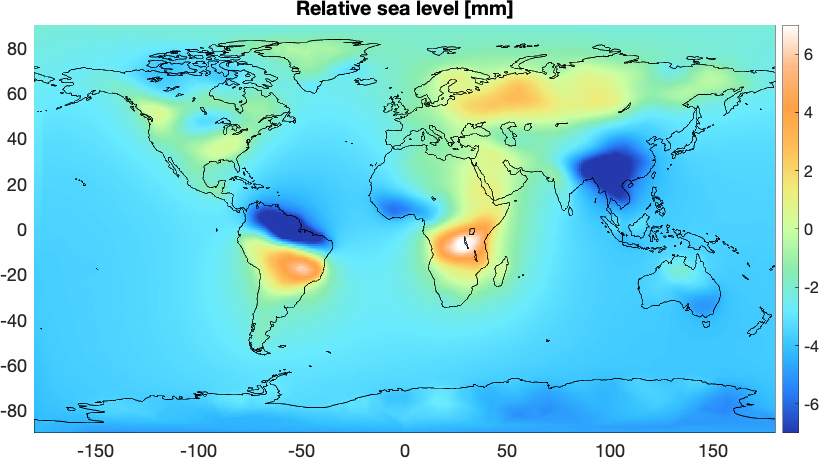
\includegraphics[scale=2]{/assets/img/tutorials/sealevelfingerprints/Rsl.png}
	\end{center}
\end{figure}
%}}}

